\chapter{Einleitung}
\section{Hintergrund}
Die Chemie im Allgemeinen befasst sich mit den Eigenschaften und Interaktionen
von Molekülen bzw. Atomen. Es ist also von hohem Interesse diese
durch akkurate Modelle zu beschreiben. In der Chemie, wie mit allen
Naturwissenschaften, wurden im Laufe der Geschichte immer genauere Theorien entwickelt.
Im 20. Jahrhundert kam es dann zur Begründung der Computerchemie durch die Einführung zweier 
revolutionärer Gebiete, die der Quantenphysik und der Informatik.
Nun war es nicht nur möglich chemische Systeme auf vorher ungesehene Genauigkeit zu beschreiben,
sondern auch noch quantitative Berechnungen mit Computern an diesen durchzuführen.
Deshalb handelt es sich bei der Computerchemie möglicherweise zukünftig
um eines der nützlichesten Werkzeuge in der Chemie.

\begin{figure}[h]
    \begin{center}
    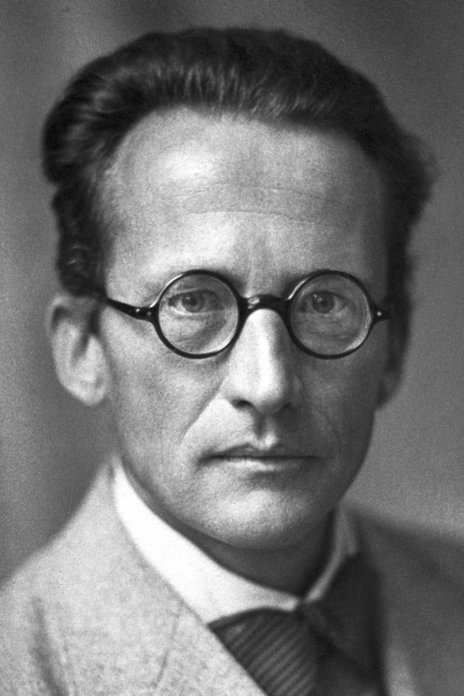
\includegraphics[width=0.25\textwidth]{res/schrodinger.jpg}
    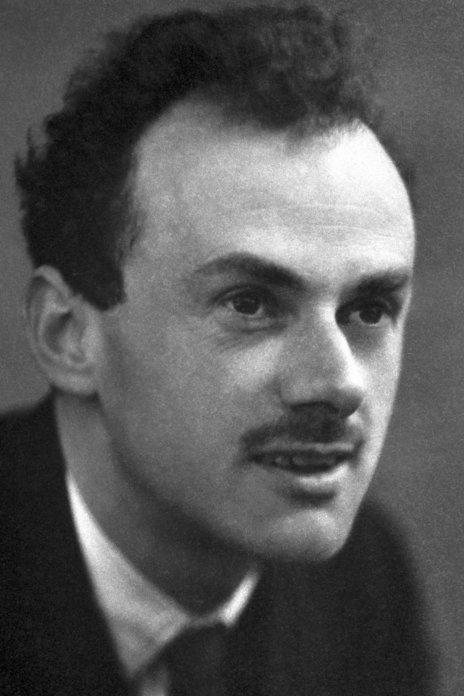
\includegraphics[width=0.25\textwidth]{res/dirac.jpg}
\end{center}
    \caption{Erwin Schrödinger und Paul Adrien Maurice Dirac wurden 1933 mit dem Nobelpreis
    für Physik ausgezeichnet für ihre Entdeckungen im Bezug auf die Atomtheorie. \cite{nobel_1933}}
\end{figure}

\section{Ziele}
Wegen der hohen Komplexität und Weitläufigkeit der Computerchemie
kann der Einstieg oft schwierig sein. Aus diesem Grund wird
in dieser Arbeit versucht eine Übersicht der notwendigen Theorie zu geben,
um selber einfache quantenchemische Berechnungen durchzuführen.
Zudem wird noch eine eigene Implementierung
zur Theorie bereitgestellt und besprochen.

Zum Einstieg bietet sich die Berechnung von wohl einer der fundamentalsten Eigenschaften 
eines Moleküls bzw. Atoms an, die Hartree\-/Fock\-/Energie, 
mit dieser können viele Prozesse in der Chemie,
wie Reaktionsabläufe und Molekülstrukturen, erklärt werden.
Um diese Energie zu berechnen, wird im Folgenden
die Hartree\-/Fock\-/Theorie entwickelt und angewendet.


\section{Einordnung der Hartee\-/Fock\-/Theorie in der Chemie} \label{posthf}
Die HF\-/Theorie gehört zur Klasse der Ab\-/Initio\-/Methoden,
welche versuchen nur basierend auf theoretischen Modellen und
universellen Konstanten Berechnung durchzuführen.
Diese Verfahren stehen im Gegensatz zu den Semiempirischen\-/Methoden,
welche zusätzliche experimentell bestimmte Werte in die Berechnungen einbinden.

Die HF-Theorie ist der einfachste noch praktisch verwendete Vertreter
der Klasse der Ab\-/Initio\-/Methoden
und wird deshalb bei entweder sonst zu großen System oder
als Start-Approximation für sehr akkurate Berechnungen verwendet.
\cite[S. 433]{structure_2013}

Basierend auf der HF-Theorie existieren die Post\-/Hartree\-/Fock\-/Methoden,
diese verbesseren die Genauigkeit der Ergebnisse hauptsächlich
durch eine genauere Behandlung der Elektron-Elektron-Interaktionen.

Neben den Post\-/HF\-/Methoden existieren zudem Verfahren
mit unterschiedlichen Ansätzen. Eine der relevantesten ist
die Dichte\-/Funktional\-/Theorie (DFT), welche nicht auf
Wellenfunktionen aufbaut sondern direkt mit den
Dichtefunktionen der Elektronen arbeitet.